\begin{figure*}[t]
\centering
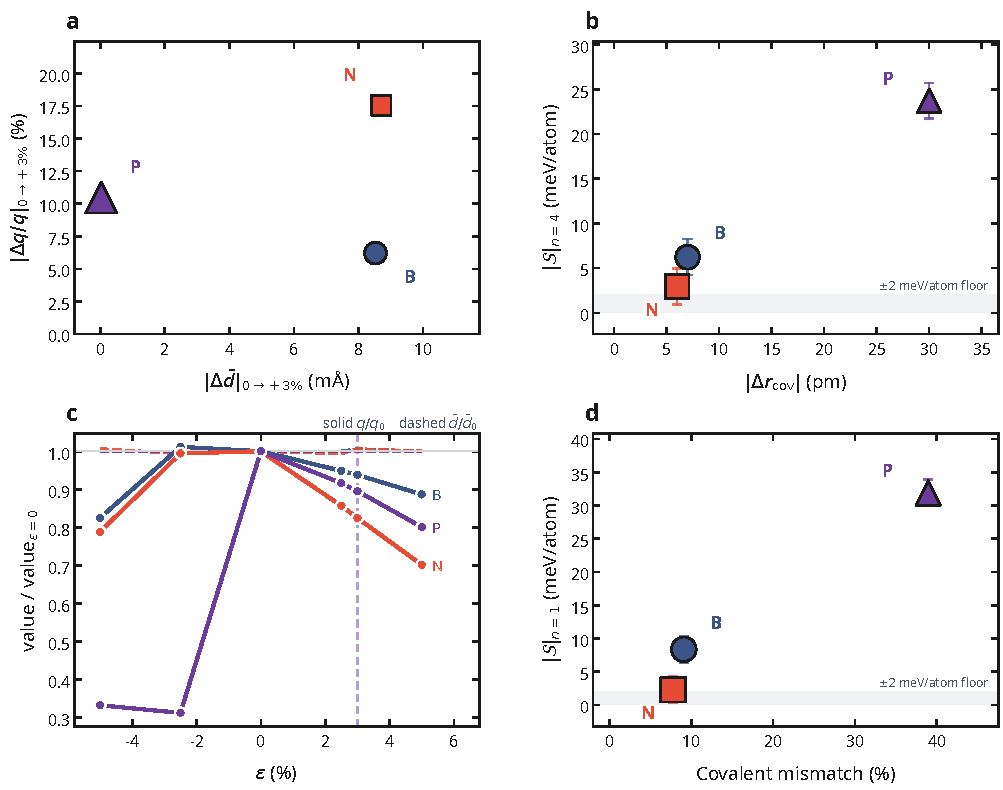
\includegraphics[width=\textwidth]{figures/out/figure_prb_4_mechanism.pdf}
\caption{\label{fig:mechanism}Schematic mechanism consistent with the present energetic and structural audits (misfit strain, charge redistribution, and $\pi$-DOS morphology are correlated observables, not a partitioned causal chain).
(a)~Response plane from $0\to{+}3$\% path endpoints; bubble area $\propto|\mathcal{S}|_{n=4}$. Neither axis orders the coupling: B and N stretch comparably ($|\Delta\bar{d}|\approx 8.5$ and $8.7$~m\AA) at intermediate and \emph{smallest} $|\mathcal{S}|$, N also redistributes the most charge ($|\Delta q/q|\approx 18$\%), and P couples most strongly while barely stretching.
(b)~$|\Delta r_{\mathrm{cov}}|$ (top axis: relative to the C covalent radius) vs.\ $|\mathcal{S}|$ at $n{=}4$ (filled) and $n{=}1$ (open); bars and band: $\pm2$~meV/atom floor. The rank follows mismatch (N $<$ B $<$ P) at both sizes, but the three points are not proportional, so radius orders without predicting magnitude. In this three-substituent audit the clearly large deviation is the largest mismatch (+30~pm, P). The panel does not mark a fitted threshold below which additivity holds.
(c)~Linked normalized paths $q(\epsilon)/q(0)$ (solid) and $\bar{d}(\epsilon)/\bar{d}(0)$ (dashed).
(d)~Parallel-coordinate summary: each observable is normalized to its maximum over B, N, P (maximum printed above each axis). P tops the mismatch and both $|\mathcal{S}|$ axes and is lowest in $|\Delta\bar d|$; N tops $|\Delta\bar d|$ (marginally above B) and $|\Delta q/q|$ and is lowest in $|\mathcal{S}|$.
With three substituents these panels are consistency checks on the misfit picture, not fitted correlations.}
\end{figure*}
